\documentclass[12pt, twoside]{article}
\usepackage[letterpaper, margin=1in, headsep=0.5in]{geometry}
\usepackage[english]{babel}
\usepackage[utf8]{inputenc}
\usepackage{amsmath}
\usepackage{amsfonts}
\usepackage{amssymb}
\usepackage{tikz}
%\usetikzlibrary{quotes, angles}

\usepackage{graphicx}
\usepackage{enumitem}
\usepackage{multicol}

\usepackage{fancyhdr}
\pagestyle{fancy}
\fancyhf{}
\renewcommand{\headrulewidth}{0pt} % disable the underline of the header

\fancyhead[RE]{\thepage}
\fancyhead[RO]{\thepage \\ Name: \hspace{3cm}}
\fancyhead[L]{BECA / Dr. Huson / 10th Grade Geometry\\* 16 January 2019}

\begin{document}
\subsubsection*{Do Now Quiz: Dilating a line segment, hexagon construction}
 \begin{enumerate}

   \item The coordinates of the endpoints of $\overline{AB}$ are $A(4,1)$ and $B(0,4)$. Determine the length of $\overline{A'B'}$, the image of  $\overline{AB}$, after a dilation of 2 centered at the origin.\\[0.25cm]
   Draw and label the two line segments,  $\overline{AB}$ and  $\overline{A'B'}$, on the set of axes below.
   \vspace{9cm}
   \begin{center}
     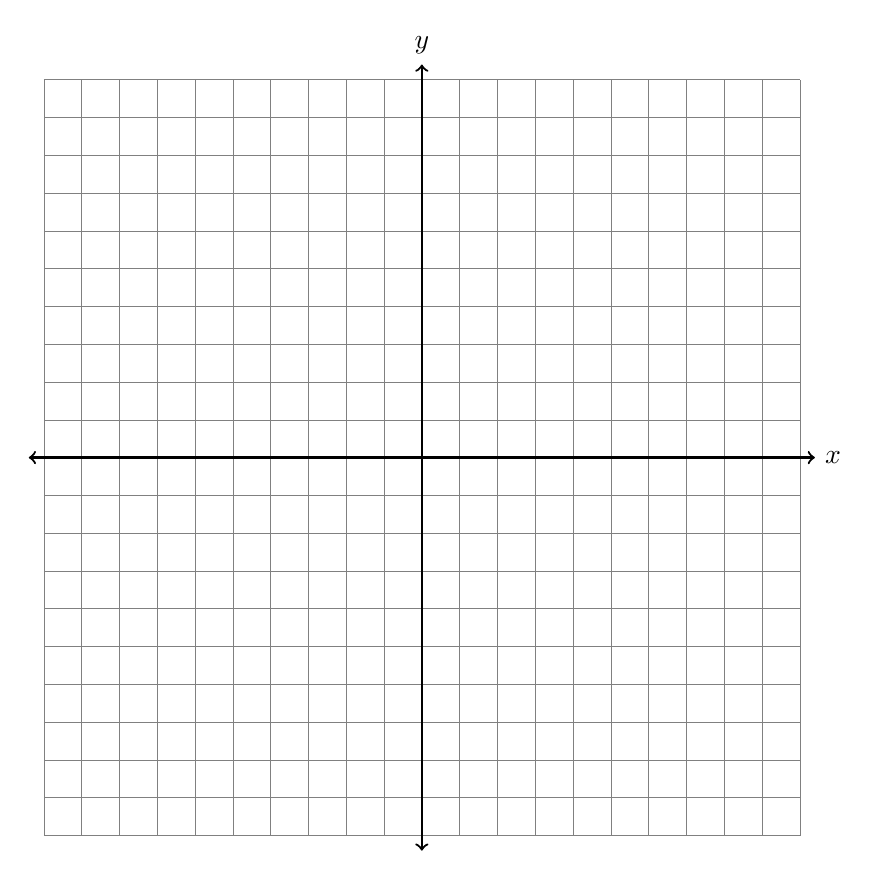
\begin{tikzpicture}[scale=.48]
       \draw [help lines] (-10,-10) grid (10,10);
       \draw [thick, <->] (-10.4,0) -- (10.4,0) node [right] {$x$};
       \draw [thick, <->] (0,-10.4)--(0,10.4) node [above] {$y$};
     \end{tikzpicture}
   \end{center}

  \newpage
  \item Regents problem:\\
  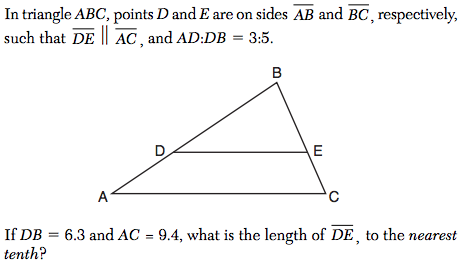
\includegraphics[width=0.7\textwidth]{similarity-ratio-spicy.png}\\[0.5cm]
  \vspace{2cm}

  \item Triangle $ADE$ and its midline $\overline{BC}$ are drawn, with $B$ the midpoint of $\overline{AD}$ and $C$ the midpoint of $\overline{AE}$. The two medians $\overline{AE}$ and $\overline{AE}$ are drawn, as shown, intersecting in point $F$, the centroid.\\[0.25cm]
  $\triangle FCB \sim \triangle FDE$ with scale factor $k=2$.\\[0.25cm]
  Given $BC=7$, find $DE$. \\[0.25cm] Given $BF=4$, find $FE$. \vspace{1cm}
  \begin{center}
      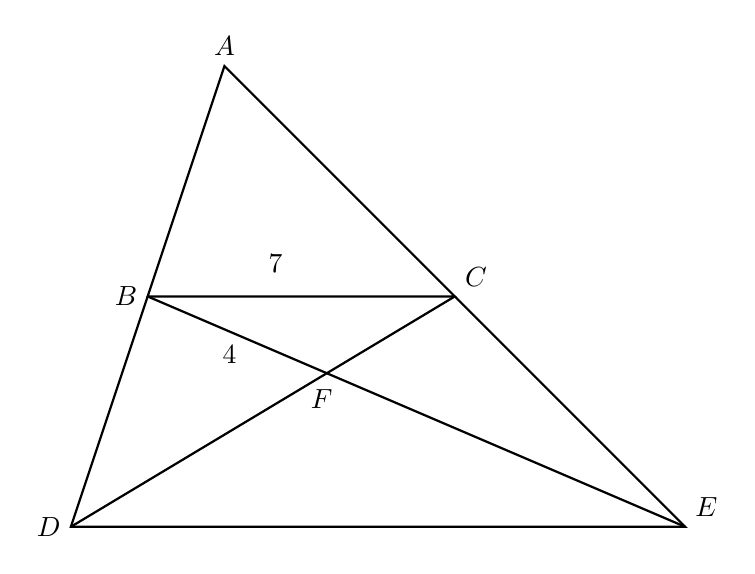
\begin{tikzpicture}[scale=0.65]
        \draw [thick]
        (0.5,1.5)node[left]{$B$}--
        (6.5,1.5)node[above right]{$C$}--
        (2,6)node[above]{$A$}--cycle;
        \draw [thick]
        (0.5,1.5)--
        (-1,-3)node[left]{$D$}--
        (11,-3)node[above right]{$E$}--(6.5,1.5);
        \draw [thick] (0.5,1.5)--(11,-3);
        \draw [thick] (6.5,1.5)--(-1,-3);
        \node at (3,2.5)[below]{$7$};
        \node at (3.5, -0.5)[right]{$F$};
        \node at (2.1, 0)[above]{$4$};
        %\node at (-0.7, -1)[above]{$5$};
      \end{tikzpicture}
    \end{center}



\end{enumerate}
\end{document}
